% Options for packages loaded elsewhere
\PassOptionsToPackage{unicode}{hyperref}
\PassOptionsToPackage{hyphens}{url}
%
\documentclass[
]{article}
\title{Data Visualization With Stata}
\author{Andy Grogan-Kaylor}
\date{\{\{.1\}\} \{\{.2\}\}}

\usepackage{amsmath,amssymb}
\usepackage{stata}
\usepackage{lmodern}
\usepackage{iftex}
\ifPDFTeX
  \usepackage[T1]{fontenc}
  \usepackage[utf8]{inputenc}
  \usepackage{textcomp} % provide euro and other symbols
\else % if luatex or xetex
  \usepackage{unicode-math}
  \defaultfontfeatures{Scale=MatchLowercase}
  \defaultfontfeatures[\rmfamily]{Ligatures=TeX,Scale=1}
\fi
% Use upquote if available, for straight quotes in verbatim environments
\IfFileExists{upquote.sty}{\usepackage{upquote}}{}
\IfFileExists{microtype.sty}{% use microtype if available
  \usepackage[]{microtype}
  \UseMicrotypeSet[protrusion]{basicmath} % disable protrusion for tt fonts
}{}
\makeatletter
\@ifundefined{KOMAClassName}{% if non-KOMA class
  \IfFileExists{parskip.sty}{%
    \usepackage{parskip}
  }{% else
    \setlength{\parindent}{0pt}
    \setlength{\parskip}{6pt plus 2pt minus 1pt}}
}{% if KOMA class
  \KOMAoptions{parskip=half}}
\makeatother
\usepackage{xcolor}
\IfFileExists{xurl.sty}{\usepackage{xurl}}{} % add URL line breaks if available
\IfFileExists{bookmark.sty}{\usepackage{bookmark}}{\usepackage{hyperref}}
\hypersetup{
  pdftitle={Data Visualization With Stata},
  pdfauthor={Andy Grogan-Kaylor},
  hidelinks,
  pdfcreator={LaTeX via pandoc}}
\urlstyle{same} % disable monospaced font for URLs
\usepackage[margin=1 in]{geometry}
\usepackage{graphicx}
\makeatletter
\def\maxwidth{\ifdim\Gin@nat@width>\linewidth\linewidth\else\Gin@nat@width\fi}
\def\maxheight{\ifdim\Gin@nat@height>\textheight\textheight\else\Gin@nat@height\fi}
\makeatother
% Scale images if necessary, so that they will not overflow the page
% margins by default, and it is still possible to overwrite the defaults
% using explicit options in \includegraphics[width, height, ...]{}
\setkeys{Gin}{width=\maxwidth,height=\maxheight,keepaspectratio}
% Set default figure placement to htbp
\makeatletter
\def\fps@figure{htbp}
\makeatother
\setlength{\emergencystretch}{3em} % prevent overfull lines
\providecommand{\tightlist}{%
  \setlength{\itemsep}{0pt}\setlength{\parskip}{0pt}}
\setcounter{secnumdepth}{-\maxdimen} % remove section numbering
\ifLuaTeX
  \usepackage{selnolig}  % disable illegal ligatures
\fi

\begin{document}
\maketitle

\hypertarget{introduction}{%
\section{Introduction}\label{introduction}}

\begin{itemize}
\tightlist
\item
  Stata is a powerful and intuitive data analysis program.
\item
  Learning how to graph in Stata is an important part of learning how to
  use Stata. Yet, the default graphs in Stata can sometimes be less than
  optimal.
\item
  This document is an introduction to (a) basic graphing ideas in Stata;
  and (b) some simple ways to make your Stata graphs look more
  professional.
\item
  If this document is presented as slides, navigation links are in the
  corner of this slide deck.
\item
  If this document is presented as slides, you can generate a printable
  version of these slides, by clicking on the ``Ø''.
\end{itemize}

\hypertarget{what-are-variables}{%
\section{What are Variables?}\label{what-are-variables}}

\begin{itemize}
\tightlist
\item
  By variables, I simply mean the columns of data that you have.
\item
  For our purposes, you may think of variables as synonymous with
  questionnaire items, or columns of data.
\end{itemize}

\hypertarget{variable-types}{%
\section{Variable Types}\label{variable-types}}

\begin{itemize}
\tightlist
\item
  \emph{categorical variables} represent unordered categories like
  \emph{neighborhood}, or \emph{religious affiliation}, or \emph{place
  of residence}.
\item
  \emph{continuous variables} represent a continuous scale like a
  \emph{mental health scale}, or a \emph{measure of life expectancy}.
\end{itemize}

\hypertarget{a-data-visualization-strategy}{%
\section{A Data Visualization
Strategy}\label{a-data-visualization-strategy}}

Once we have discerned the type of variable that have, there are two
followup questions we may ask before deciding upon a chart strategy:

\begin{itemize}
\tightlist
\item
  Is our graph about \textbf{one thing at a time}?

  \begin{itemize}
  \tightlist
  \item
    How much of \emph{x} is there?
  \item
    What is the distribution of \emph{x}?
  \end{itemize}
\item
  Is our graph about \textbf{two things at a time}?

  \begin{itemize}
  \tightlist
  \item
    What is the relationship of \emph{x} and \emph{y}?
  \item
    How are \emph{x} and \emph{y} associated?
  \end{itemize}
\end{itemize}

\hypertarget{data}{%
\section{Data}\label{data}}

We are going to use the famous ``iris'' data collected by Edgar Anderson
in the early 20th Century.

\begin{stlog}
. use "iris.dta", clear
{\smallskip}
. 
. summarize
{\smallskip}
    Variable {\VBAR}        Obs        Mean    Std. dev.       Min        Max
\HLI{13}{\PLUS}\HLI{57}
Sepal_Length {\VBAR}        150    5.843333    .8280661        4.3        7.9
 Sepal_Width {\VBAR}        150    3.057333    .4358663          2        4.4
Petal_Length {\VBAR}        150       3.758    1.765298          1        6.9
 Petal_Width {\VBAR}        150    1.199333    .7622377         .1        2.5
     Species {\VBAR}        150           2    .8192319          1          3
\end{stlog}

\begin{quote}
The \texttt{iris} data set has 5 variables.
\end{quote}

\hypertarget{species-of-iris}{%
\section{Species of Iris}\label{species-of-iris}}

\begin{quote}
Iris species images courtesy
\href{https://www.wikipedia.org/}{Wikipedia}.
\end{quote}

\begin{figure}
\centering
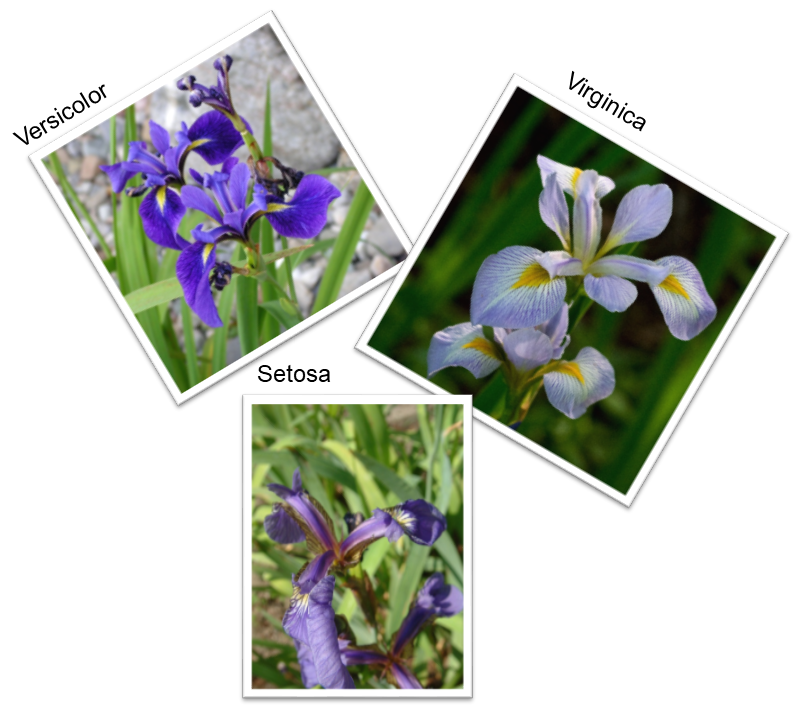
\includegraphics[width=0.75\linewidth]{iris-species.png}
\caption{Iris Species}
\end{figure}

\hypertarget{petals-and-sepals}{%
\section{Petals and Sepals}\label{petals-and-sepals}}

\begin{figure}
\centering
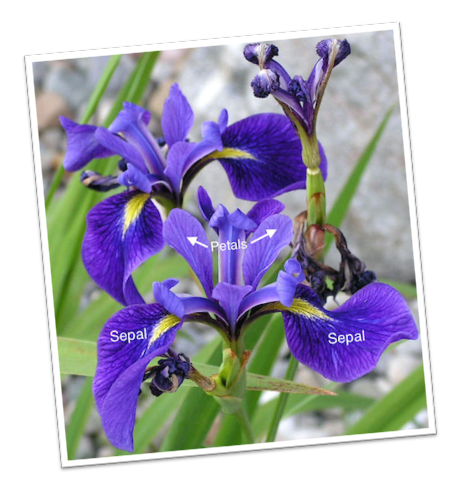
\includegraphics[width=0.75\linewidth]{petal-sepal.png}
\caption{Petals and Sepals}
\end{figure}

\hypertarget{basic-graphs}{%
\section{Basic Graphs}\label{basic-graphs}}

\hypertarget{continuous-variable-histogram}{%
\section{\texorpdfstring{Continuous Variable
\texttt{histogram}}{Continuous Variable histogram}}\label{continuous-variable-histogram}}

\begin{stlog}
. histogram Petal_Length
(bin=12, start=1, width=.49166667)
\end{stlog}



\begin{figure}
\centering
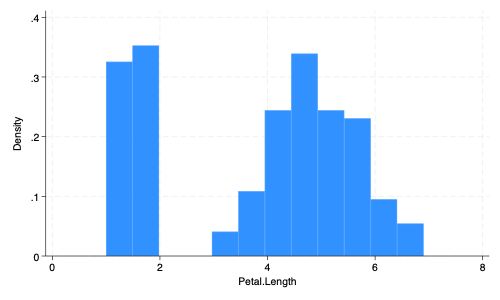
\includegraphics[width=0.75\linewidth]{myhistogram.png}
\caption{Histogram of Petal Width}
\end{figure}

\hypertarget{categorical-variable-graph-bar}{%
\section{\texorpdfstring{Categorical Variable
\texttt{graph\ bar}}{Categorical Variable graph bar}}\label{categorical-variable-graph-bar}}

\begin{stlog}
. graph bar, over(Species)
\end{stlog}



\begin{figure}
\centering
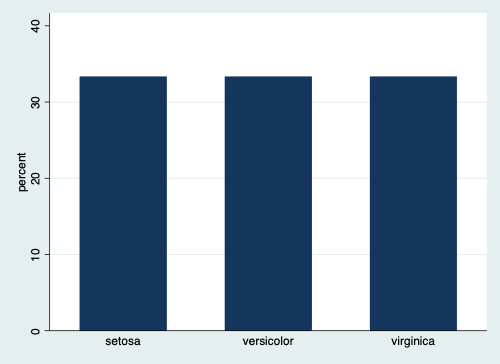
\includegraphics[width=0.75\linewidth]{mybargraph.png}
\caption{Bar Graph of Species}
\end{figure}

\hypertarget{continuous-by-continuous-twoway}{%
\section{\texorpdfstring{Continuous by Continuous
\texttt{twoway}}{Continuous by Continuous twoway}}\label{continuous-by-continuous-twoway}}

\begin{stlog}
. twoway scatter Petal_Length Petal_Width
\end{stlog}



\begin{figure}
\centering
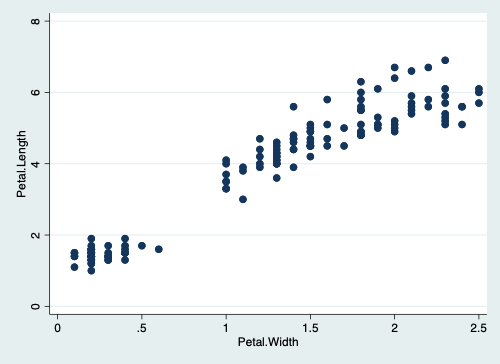
\includegraphics[width=0.75\linewidth]{myscatter.png}
\caption{Scatterplot}
\end{figure}

\hypertarget{categorical-by-categorical-graph-bar}{%
\section{\texorpdfstring{Categorical by Categorical
\texttt{graph\ bar}}{Categorical by Categorical graph bar}}\label{categorical-by-categorical-graph-bar}}

\begin{stlog}
. recode Petal_Length ///
> (min/3.758 = 0 "below mean") ///
> (3.758/max = 1 "above mean"), ///
> generate(Petal_Group) // dichotomize Petal_Length
(150 differences between {\bftt{Petal_Length}} and {\bftt{Petal_Group}})
{\smallskip}
.     
. graph bar, over(Species) over(Petal_Group)
\end{stlog}



\begin{figure}
\centering
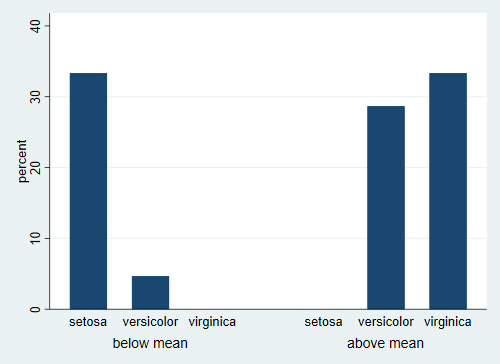
\includegraphics[width=0.75\linewidth]{mybargraph2.png}
\caption{Bar Graph of Species by Category of Petal Length}
\end{figure}

\hypertarget{continuous-by-categorical-graph-bar}{%
\section{\texorpdfstring{Continuous by Categorical
\texttt{graph\ bar}}{Continuous by Categorical graph bar}}\label{continuous-by-categorical-graph-bar}}

\begin{stlog}
. graph bar Petal_Length, over(Species)
\end{stlog}



\begin{figure}
\centering
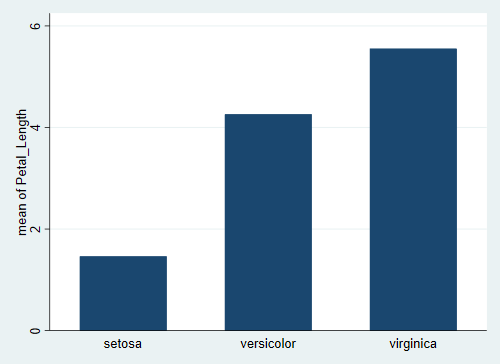
\includegraphics[width=0.75\linewidth]{mybargraph3.png}
\caption{Bar Graph of Petal Length by Species}
\end{figure}

\hypertarget{titles-and-labels-title...-xtitle...-ytitle...}{%
\section{\texorpdfstring{Titles and Labels
\texttt{,\ title(...)\ xtitle(...)\ ytitle(...)}}{Titles and Labels , title(...) xtitle(...) ytitle(...)}}\label{titles-and-labels-title...-xtitle...-ytitle...}}

\begin{stlog}
. twoway scatter Petal_Length Petal_Width, scheme(s1rcolor) ///
> title("Petal Length by Petal Width") ///
> xtitle("Petal Width") ytitle("Petal Width") ///
> caption("Iris Data") 
\end{stlog}



\begin{figure}
\centering
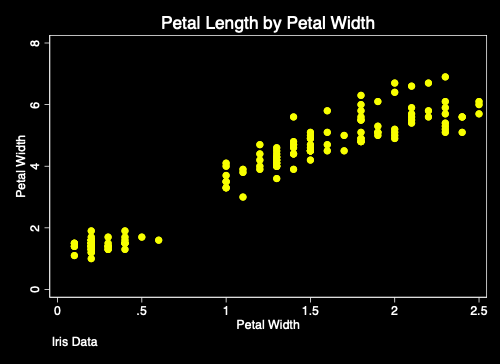
\includegraphics[width=0.75\linewidth]{graphtitleslabels.png}
\caption{Graph With Titles and Labels}
\end{figure}

\hypertarget{better-graphing-with-schemes-scheme...}{%
\section{\texorpdfstring{Better Graphing With Schemes
\texttt{,scheme(...)}}{Better Graphing With Schemes ,scheme(...)}}\label{better-graphing-with-schemes-scheme...}}

The easiest method to make better Stata graphs is through the use of
predefined Stata graphing schemes.

\hypertarget{pre-defined-schemes}{%
\section{Pre-Defined Schemes}\label{pre-defined-schemes}}

Some schemes, e.g.~\texttt{economist}, \texttt{sj}, \texttt{s1color},
and \texttt{s1rcolor} are pre-installed with Stata.

\hypertarget{economist-scheme}{%
\section{Economist Scheme}\label{economist-scheme}}

\begin{stlog}
. twoway scatter Petal_Length Petal_Width, scheme(economist)
\end{stlog}



\begin{figure}
\centering
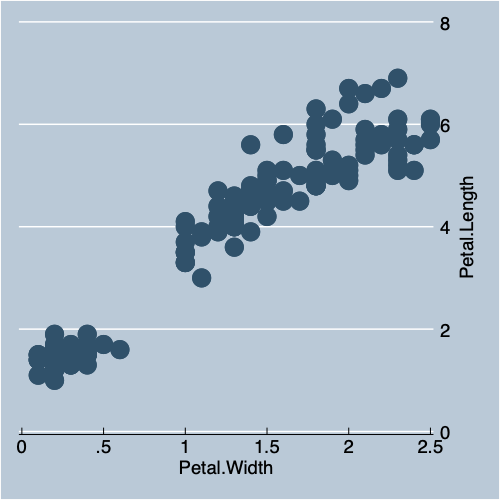
\includegraphics[width=0.75\linewidth]{econscatter.png}
\caption{Scatterplot with Economist Scheme}
\end{figure}

\hypertarget{stata-journal-scheme}{%
\section{\texorpdfstring{\emph{Stata Journal}
Scheme}{Stata Journal Scheme}}\label{stata-journal-scheme}}

\begin{stlog}
. twoway scatter Petal_Length Petal_Width, scheme(sj)
\end{stlog}



\begin{figure}
\centering
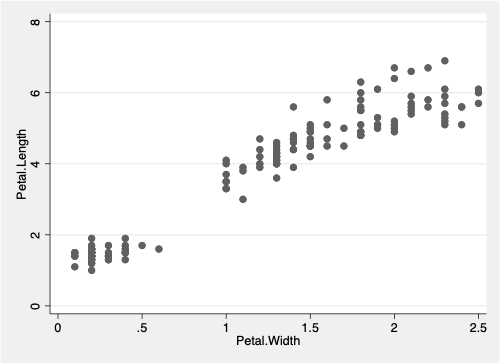
\includegraphics[width=0.75\linewidth]{sjscatter.png}
\caption{Scatterplot with \emph{Stata Journal} Scheme}
\end{figure}

\hypertarget{s1color-scheme}{%
\section{\texorpdfstring{\texttt{s1color}
Scheme}{s1color Scheme}}\label{s1color-scheme}}

\begin{stlog}
. twoway scatter Petal_Length Petal_Width, scheme(s1color)
\end{stlog}



\begin{figure}
\centering
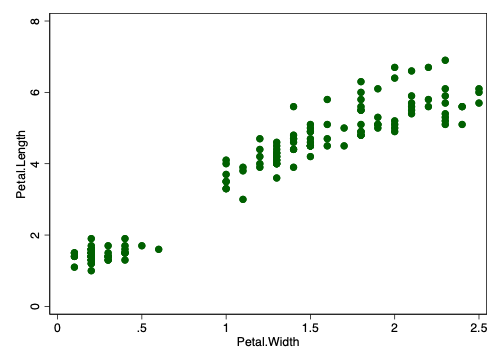
\includegraphics[width=0.75\linewidth]{s1colorscatter.png}
\caption{Scatterplot with \texttt{s1color} Scheme}
\end{figure}

\hypertarget{s1rcolor-scheme}{%
\section{\texorpdfstring{\texttt{s1rcolor}
Scheme}{s1rcolor Scheme}}\label{s1rcolor-scheme}}

\begin{stlog}
. twoway scatter Petal_Length Petal_Width, scheme(s1rcolor)
\end{stlog}



\begin{figure}
\centering
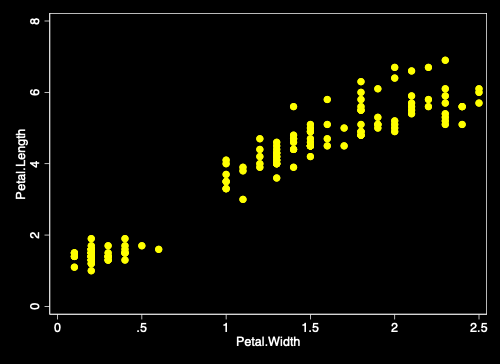
\includegraphics[width=0.75\linewidth]{s1rcolorscatter.png}
\caption{Scatterplot with \texttt{s1rcolor} Scheme}
\end{figure}

\hypertarget{user-written-schemes}{%
\section{User Written Schemes}\label{user-written-schemes}}

Two of the best user written schemes are \texttt{plottig} and
\texttt{lean2}.

Use the \texttt{findit} command e.g.~\texttt{findit\ lean2} to find
these schemes.

\hypertarget{lean2-scheme}{%
\section{\texorpdfstring{\texttt{lean2}
Scheme}{lean2 Scheme}}\label{lean2-scheme}}

\begin{stlog}
. twoway scatter Petal_Length Petal_Width, scheme(lean2)
\end{stlog}



\begin{figure}
\centering
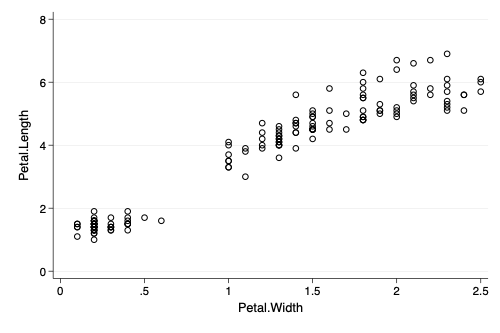
\includegraphics[width=0.75\linewidth]{lean2scatter.png}
\caption{Scatterplot with \texttt{lean2} Scheme}
\end{figure}

\hypertarget{michigan-graph-scheme}{%
\section{Michigan graph scheme}\label{michigan-graph-scheme}}

I have written a \texttt{michigan} graph scheme described
\href{https://agrogan1.github.io/Stata/}{here}.

\begin{stlog}
. twoway (scatter Petal_Length Petal_Width) /// 
> (lfit Petal_Length Petal_Width), scheme(michigan)
\end{stlog}



\begin{figure}
\centering
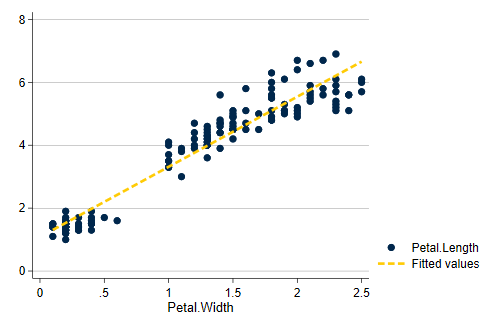
\includegraphics[width=0.75\linewidth]{michiganscatter.png}
\caption{Scatterplot with \texttt{michigan} Scheme}
\end{figure}

\hypertarget{schemes-as-a-base-for-further-tweaking}{%
\section{Schemes as a Base for Further
Tweaking}\label{schemes-as-a-base-for-further-tweaking}}

Schemes can be used as a base that can then be further modified.

\begin{stlog}
. twoway (scatter Petal_Length Petal_Width, msymbol(0) mcolor(red)) ///
> (lfit Petal_Length Petal_Width), ///
> scheme(lean2) 
(note:  named style 0 not found in class symbol, default attributes used)
\end{stlog}



\begin{figure}
\centering
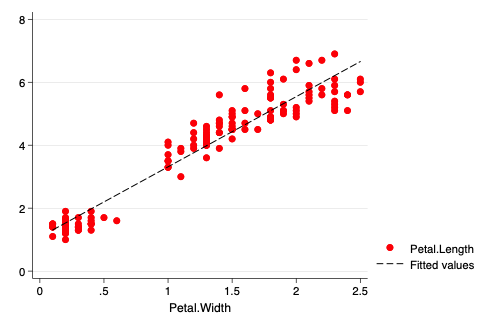
\includegraphics[width=0.75\linewidth]{lean2Ascatter.png}
\caption{Modified Scatterplot with \texttt{lean2} Scheme as a Base}
\end{figure}

\hypertarget{even-more-tweaks}{%
\section{Even More Tweaks}\label{even-more-tweaks}}

Based upon an example at
\url{https://blog.stata.com/2018/10/02/scheming-your-way-to-your-favorite-graph-style/}

\begin{stlog}
. twoway scatter Sepal_Length Sepal_Width Petal_Width Petal_Length, /// 
> color(\%50 \%50 \%50) /// transparency 
> title("Multiple Iris Characteristics") /// title
> scheme(s1rcolor) // scheme
\end{stlog}



\begin{figure}
\centering
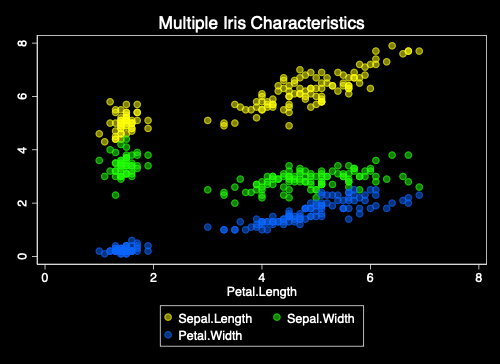
\includegraphics[width=0.75\linewidth]{s1rcolorAscatter.png}
\caption{Modified Scatterplot with \texttt{s1rcolor} Scheme as a Base}
\end{figure}

\hypertarget{more-information}{%
\section{More Information}\label{more-information}}

See also
\href{https://agrogan1.github.io/Stata/two-page-stata/TwoPageStata.pdf}{Two
Page Stata}

Created by \url{agrogan@umich.edu}

\end{document}
